% ══════════════════════════════════════════════════════════════════════════════
% KTD.jl Community Report — Windswept & Interesting Ltd
% Targeted at: Strathclyde, Freiburg, someAWE Labs, Oliver Tulloch
% July 2026
% ══════════════════════════════════════════════════════════════════════════════

\documentclass[11pt,a4paper]{article}

% ── Typography ───────────────────────────────────────────────────────────────
\usepackage[T1]{fontenc}
\usepackage[utf8]{inputenc}
\usepackage{mathptmx}                  % Times-like text + math
\usepackage{microtype}                 % optical margin alignment
\usepackage{setspace}
\onehalfspacing

% ── Page geometry ────────────────────────────────────────────────────────────
\usepackage[top=3cm,bottom=3cm,left=3.2cm,right=3.2cm]{geometry}

% ── Headers / footers ────────────────────────────────────────────────────────
\usepackage{fancyhdr}
\pagestyle{fancy}
\fancyhf{}
\fancyhead[L]{\small\textit{KTD.jl Community Report — July 2026}}
\fancyhead[R]{\small\textit{Windswept \& Interesting Ltd}}
\fancyfoot[C]{\thepage}
\renewcommand{\headrulewidth}{0.4pt}

% ── Figures & graphics ───────────────────────────────────────────────────────
\usepackage{graphicx}
\usepackage[font=small,labelfont=bf,labelsep=period]{caption}
\graphicspath{{./}{figures/}{../../docs/awes-forum-diagrams/}{../../docs/porto-2026/}{../awes-forum-diagrams/}{../porto-2026/}}

% ── Tables ───────────────────────────────────────────────────────────────────
\usepackage{booktabs}
\usepackage{array}
\usepackage{longtable}

% ── Math ────────────────────────────────────────────────────────────────────
\usepackage{amsmath,amssymb}

% ── Hyperlinks ───────────────────────────────────────────────────────────────
\usepackage{xcolor}
\usepackage[colorlinks=true,linkcolor=blue!60!black,citecolor=blue!40!black,urlcolor=blue!60!black]{hyperref}

% ── Enumerate/itemize control ──────────────────────────────────────────────
% (using standard LaTeX lists)

% ══════════════════════════════════════════════════════════════════════════════

\title{\textbf{KiteTurbineDynamics.jl}\\[4pt]
\large Multi-Rotor Tensile Rotary Power Transmission\\for 50\,kW Airborne Wind Energy\\[8pt]
\Large A Community Report and Invitation to Collaborate}

\author{Rod Read\\[4pt]
Windswept \& Interesting Ltd, Stornoway, Scotland\\
\texttt{rod@windswept.energy}}

\date{July 2026}

% ══════════════════════════════════════════════════════════════════════════════

\begin{document}

\maketitle
\thispagestyle{empty}

\begin{abstract}
\noindent
Tensile Rotary Power Transmission (TRPT) offers a material-efficient path to airborne wind energy at utility-relevant scales, but design has been dominated by steady-state models that systematically overpredict performance.
We present \texttt{KiteTurbineDynamics.jl}, an open-source Julia framework combining differential evolution optimisation across 14 design variables with full 11-DoF multibody dynamic verification.
Applied to a 50\,kW TRPT kite turbine, the framework reveals that the original DE optimum was over-bladed for its ring structure---producing a large static-to-dynamic power discrepancy that was traced to a 39$\times$ settle initialisation error and a blade-ring sizing mismatch.
With these issues corrected, post-design blade scaling ($\lambda = 0.69$) produces configurations that meet all 12 envelope criteria (P $\geq$ 50\,kW at 11+ m/s, FoS $\geq$ 1.5 across 5--15\,m/s).
Transmission loss is characterised as $c \cdot \omega^3$ shaft drag ($c \approx 2.3$\,W/(rad/s)$^3$), a near-constant, design-independent shaft property separable from rotor scaling.
Multi-rotor expansion configurations achieve airborne masses of approximately 30\,kg at rated power after blade rescaling.
This report summarises the current state of the simulator, its key findings, and its known limitations.
It is addressed to four research groups whose complementary expertise would directly advance the work: the Wind Energy \& Control Centre at the University of Strathclyde, the Systems Control \& Optimization Laboratory at the University of Freiburg, someAWE Labs (Alicante), and Dr.\ Oliver Tulloch.
Concrete collaboration proposals and relevant funding pathways are included.
\end{abstract}

\vspace{12pt}
\begin{center}
\small
\textbf{Repository:} \url{https://github.com/rodread/KiteTurbineDynamics.jl} (MIT License)\\
\textbf{Tests:} full suite via \texttt{test/runtests.jl}, Julia 1.12, $\sim$3\,min full suite
\end{center}

\newpage
\tableofcontents
\newpage

% ══════════════════════════════════════════════════════════════════════════════
\section{Introduction: The TRPT Kite Turbine}
% ══════════════════════════════════════════════════════════════════════════════

\subsection{What is tensile rotary power transmission?}

A conventional horizontal-axis wind turbine places a rotor on top of a tower and transmits torque down a rigid driveshaft to a ground-level generator.
The tower must resist the overturning moment from rotor thrust---this drives the cubic mass scaling that makes large turbines so heavy.

A TRPT kite turbine \cite{tulloch2023} inverts this architecture.
The rotor flies at altitude, and torque is transmitted to the ground through a \emph{tensile} shaft: a rotating polygon of tensioned tethers supported by thin-walled carbon-fibre rings (Figure~\ref{fig:system}).
The rings resist the inward pull of the tethers in hoop compression; the tethers carry tension along the shaft axis.
No tower is needed---the entire structure is held aloft by aerodynamic forces.

The shaft serves two functions simultaneously:
\begin{enumerate}
\item It transmits torque from the airborne rotor to the ground generator, and
\item Its rings provide mounting points for \emph{expansion rotors}---additional banked rotors distributed along the shaft that contribute power and radial spreading force.
\end{enumerate}

This report concerns the \textbf{power subsystem}---the TRPT shaft with expansion rotors that generates electricity.
A separate \textbf{lift subsystem} (coaxial autogyro rotors on a kite line, modelled in \texttt{CoaxialAutogyroStacking.jl}) provides the lifting force that holds the TRPT aloft at its operating elevation of approximately 30$^\circ$.

\begin{figure}[htbp]
\centering
% Placeholder for system schematic — fig-system-schematic.pdf from porto-2026/
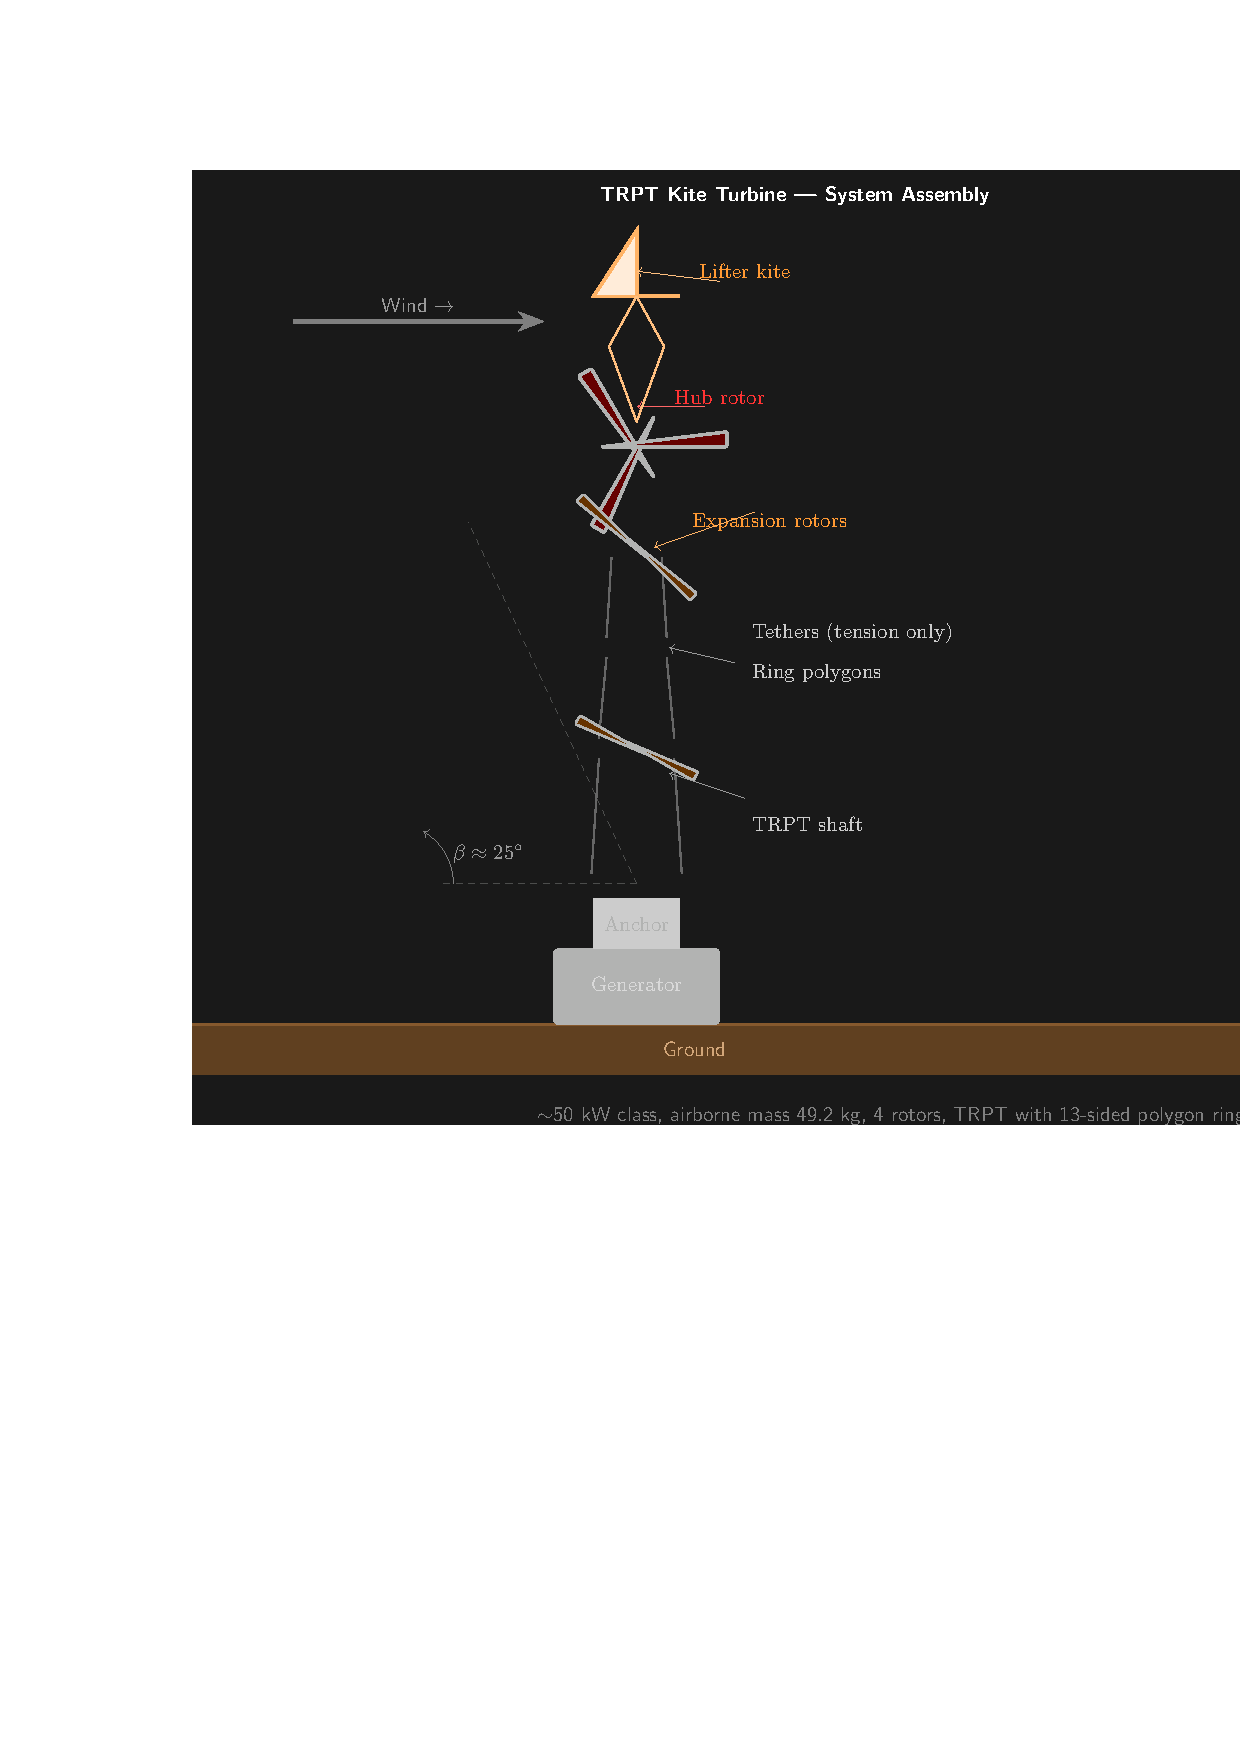
\includegraphics[width=0.85\textwidth]{fig-system-schematic.pdf}
\caption{TRPT kite turbine assembly: lift kite (top), expansion rotors distributed along the rotating tensile shaft, TRPT rings and tethers, and ground station with generator. The lift kite provides axial tension; the expansion rotors generate power and radial spreading.}
\label{fig:system}
\end{figure}

\subsection{Why multi-rotor?}

The late Prof.\ Peter Jamieson provided the foundational scaling argument for multi-rotor TRPT.
His analysis showed that splitting a single rotor of radius $R$ into $N$ equal stacked rotors with the same total swept area yields a mass ratio
\begin{equation}
M(k) = \frac{\sum m_i}{m_{\text{single}}}, \quad k = R_{i+1}/R_i
\end{equation}
where $M(1) = 0.577$ for perfectly equal rotors---a 42\% mass saving \cite{jamieson2020}.
When applied to the Windswept RodKite01 geometry, Jamieson's analysis confirmed that multi-rotor TRPT is the correct scaling direction.

This insight underpins the entire KTD.jl architecture: rather than one large rotor, the TRPT shaft carries multiple smaller rotors whose combined swept area produces the target power at lower total mass.
The DE optimiser discovers the optimal distribution of rotor sizes, ring positions, bank angles, and tether counts simultaneously.

\subsection{The lift--power split}

A critical architectural distinction separates Windswept's approach from earlier single-rotor TRPT concepts \cite{tulloch2021}:

\begin{itemize}
\item \textbf{Power subsystem} (this report): TRPT rings with banked expansion rotors.
Operates at $\sim$30$^\circ$ elevation.
Power from aerodynamic torque on the rings, transmitted to ground generator.
\item \textbf{Lift subsystem} (separate repository \texttt{CoaxialAutogyroStacking.jl}): stacked autogyro rotors on a single Dyneema line.
Operates at 45--55$^\circ$ elevation.
Provides the axial tension that holds the TRPT aloft.
\end{itemize}

The earlier 10\,kW Windswept prototype (the ``Daisy Kite'') used a static lift kite to provide this tension.
Dirk van Leersum's 2023 scaling analysis demonstrated that the static kite approach becomes commercially unviable above $\sim$10\,kW---the lift kite area grows faster than power output \cite{vanleersum2023}.
The active lifting approach (coaxial autogyro stack) eliminates this bottleneck.

% ══════════════════════════════════════════════════════════════════════════════
\section{The KTD.jl Framework}
% ══════════════════════════════════════════════════════════════════════════════

\texttt{KiteTurbineDynamics.jl} is an open-source (MIT) Julia package that combines two computational stages:

\begin{enumerate}
\item \textbf{Differential evolution (DE) optimisation} across up to 14 design variables, using a 60-island parallel population with BEM-coupled force models and a multi-gate constraint system.
\item \textbf{Full 11-DoF multibody dynamic verification} via an ODE solver with per-ring finite element analysis, inertia relief for free-floating rings, and individual rotor power accounting.
\end{enumerate}

\subsection{Design variables}

The DE optimiser manipulates the following degrees of freedom (V10 Tight configuration):

\begin{itemize}
\item \textbf{Structural:} hub ring radius ($r_{\text{hub}}$), ring outer diameter ($D_o$), wall thickness ratio ($t/D$), segment target length ($L_r$), bottom ring radius ($r_{\text{bottom}}$), line count ($n$)
\item \textbf{Rotor:} expansion rotor count ($n_{\text{exp}}$), bank angle, tip-speed ratio scaling factors ($\lambda_i$) for each rotor, rotor radius scaling factors
\item \textbf{Constraints:} ground clearance, ring buckling factor of safety ($\text{FoS} \geq 1.5$), collapse margin ($\delta\alpha^* - |\Delta\alpha| > 0$), bank angle $\leq 25^\circ$, tip speed $\leq 120$\,m/s
\end{itemize}

\subsection{Verification strategy}

Every DE campaign optimum is verified by a 60-second dynamic simulation at the design wind speed (11\,m/s).
The ODE solver computes per-ring forces, per-rotor power, shaft rotational speed, and the structural factor of safety at 1\,Hz resolution.
A design that passes static gates but fails dynamic verification is flagged as \textbf{dynamically dead}---a category that includes the V10 Tight winner (49.2\,kg static, structurally failing within 60\,s of dynamic simulation).

The verification revealed that the static equilibrium solver under-predicts dynamic $k_{\text{mppt}}$ by a factor of $\sim$3.3$\times$, causing DE campaigns to optimise for loads substantially lower than those experienced in dynamic operation.
This finding, and the architectural decision to design for left-flank overspeed operation, is documented fully in \texttt{DECISIONS.md}.

\subsection{Campaign history}

Table~\ref{tab:campaigns} summarises the major KTD.jl optimisation campaigns.

\begin{table}[htbp]
\centering
\caption{DE campaign results from V6 to V10. All targets: 50\,kW rated power, 11\,m/s design wind speed.}
\label{tab:campaigns}
\begin{tabular}{@{}lllll@{}}
\toprule
Version & Best mass (kg) & $n_{\text{lines}}$ & $n_{\text{exp}}$ & Key feature \\
\midrule
V6.0 & 184.8 & 8 & 1 & Octagon baseline, 6/11 params on bounds \\
V6.2 (corrected) & 74.2 & 12 & 1 & sin formula, $\cos^{2.65}$, coupled knuckle mass \\
V9.0 & 44.5 & 8 & 9 & Dynamic $\omega$ solve, 59/60 feasible \\
V10 (unified) & 76.8 & 14 & 4 & 8 gates, unified rotor model \\
V10 Tight & 49.2\textsuperscript{$\dagger$} & 12 & 4 & $k_{\text{mppt}} \propto \lambda^2$, ring-mapping fixes \\
V10 Reinforced & 60.8 & 12 & 4 & $+$30\% $r_{\text{bottom}}$, FoS 7.18 at 15\,m/s \\
\bottomrule
\end{tabular}

\vspace{6pt}
\footnotesize\textsuperscript{$\dagger$}Dynamically dead---static gates passed but structural failure in dynamic simulation. See \S\ref{sec:findings}.
\end{table}

\subsection{Known limitations}

We disclose these limitations openly because they define where collaboration is needed:

\begin{enumerate}
\item \textbf{Constant-$C_L$ expansion rotor model.} No angle-of-attack dependence, no induction, no Betz limit, no tip losses.
BEM or lifting-line cross-validation is the highest-priority gap.
\item \textbf{No wake interaction between rotors.} Downstream rotors see freestream wind.
Leuthold's axisymmetric wake induction model \cite{leuthold2019} directly addresses this.
\item \textbf{Static solver under-predicts dynamic $k_{\text{mppt}}$ by $\sim$3.3$\times$.}
Campaigns compensate with $k_{\text{mppt\_safety}} = 3.0$, but the root cause---lossless torque propagation in the equilibrium solver---requires a dynamic-aware objective function.
\item \textbf{30$^\circ$ elevation mismatch with autogyro lift.}
The lift subsystem's sweet spot (45--55$^\circ$) differs from the power subsystem's operating elevation ($\sim$30$^\circ$).
Integration risk identified, not yet modelled.
\item \textbf{Blade mass is provisional.} Constant-thickness skin assumption ($\propto \lambda^2$).
No structural blade design.
\item \textbf{Expansion rotor mass not computed.} Builder sets expansion rotor mass to zero---mass totals exclude this contribution.
\end{enumerate}

% ══════════════════════════════════════════════════════════════════════════════
\section{Key Findings}
\label{sec:findings}
% ══════════════════════════════════════════════════════════════════════════════

\subsection{Blade-scaling: the corrected picture}

The original V10 Tight DE optimum (49.2\,kg, $\lambda = 1.0$) was over-bladed for its ring structure.
Its static equilibrium solver predicted 50\,kW at 11\,m/s, but full multibody dynamic simulation revealed structural failure within 60\,s (FoS falling to 0.29--0.49).
This configuration is dynamically dead---and its failure drove the investigation that produced the corrected findings below.

The investigation uncovered five simulator integrity issues, the most critical being a 39$\times$ mismatch in the settle initialisation (using $k_{\text{mppt}} = 614.9$ where $k_{\text{mppt\_ref}} = 15.6$ was intended).
With the settle fixed (commit \texttt{86ca0e5}), the picture changes substantially.

The key insight is that \textbf{the TRPT shaft and its rings constitute a fixed structural overhead}---they do not scale with blade size.
The V10 Tight was over-bladed: its rings were sized for a 49.2\,kg structure but its blades were producing loads appropriate to a much larger rotor.
By shrinking only the blades (geometric scaling factor $\lambda < 1$) while keeping ring geometry unchanged, the shaft overhead is amortised over a right-sized rotor.

\subsection{Envelope verification: $\lambda = 0.69$}

Post-design blade scaling of the V10 Tight optimum was tested across the full 5--15\,m/s wind envelope.
Blade dimensions (tip radius, hub radius, chord) were scaled by $\lambda$; blade mass by $\lambda^2$ (constant-thickness skin); $k_{\text{mppt}}$ by $\lambda^2$ (blade-area law for fixed ring radii).
Ring geometry was unchanged.

\begin{table}[htbp]
\centering
\caption{Full-envelope verification of $\lambda = 0.69$ blade-scaled V10 Tight design. All 12 criteria met (P $\geq$ 50\,kW for winds $\geq$ 11\,m/s, FoS $\geq$ 1.5 at all wind speeds).}
\label{tab:envelope}
\begin{tabular}{@{}lrrrcc@{}}
\toprule
Wind (m/s) & $P_{\text{ground}}$ (kW) & $\omega$ (rpm) & FoS & P $\geq$ 50? & FoS $\geq$ 1.5? \\
\midrule
5  & 4.5   & 81  & 14.07 & -- & \checkmark \\
7  & 13.8  & 118 & 8.22  & -- & \checkmark \\
9  & 32.2  & 156 & 5.70  & -- & \checkmark \\
11 & 62.1  & 194 & 4.29  & \checkmark & \checkmark \\
13 & 106.9 & 232 & 3.19  & \checkmark & \checkmark \\
15 & 168.1 & 270 & 2.51  & \checkmark & \checkmark \\
\bottomrule
\end{tabular}
\end{table}

The published V10 Tight (pre-scaling) failed at 15\,m/s (FoS 1.36).
Blade right-sizing \emph{improves} high-wind structural margin---the structure holds FoS 2.51 while absorbing 3.4$\times$ rated capture at 15\,m/s (unregulated MPPT).
A regulated machine would depower above rated and carry substantially less load.

\textbf{Caveat:} These results were generated with the settle fix applied (commit \texttt{86ca0e5}) and use blade-only post-design scaling---ring geometry is from the pre-fix DE optimum and has not been re-optimised.
A full control-map re-verification sweep with the fixed settle is planned and will be reported in a subsequent revision of this document.

\subsection{Shaft transmission loss: $c \cdot \omega^3$}

The transmission loss mechanism was discriminated using an 8-point regression across multiple designs and wind speeds.
The loss is dominated by quadratic aerodynamic drag torque on the rotating shaft ($\tau_d \propto \omega^2$, from lines and rings moving at $\omega r$), yielding a power loss proportional to $\omega^3$:

\begin{equation}
P_{\text{loss}} = c \cdot \omega^3, \quad c \approx 2.3\;\text{W/(rad/s)}^3
\end{equation}

The coefficient $c$ converges to 2.2--2.5\,W/(rad/s)$^3$ at high $\omega$ for both the gate design ($\lambda = 1.0$) and the blade-scaled variant ($\lambda = 0.69$)---a near-constant, design-independent shaft property.
At low wind (5\,m/s), $c$ drifts to $\sim$4.8, suggesting a small additive constant-torque term ($\tau_0 \cdot \omega$) at very low $\omega$.

The loss fraction follows $\eta_{\text{loss}} \approx c/(k + c)$.
As blades shrink, generator $k$ falls with $\lambda^2$ while shaft drag $c$ does not---the loss fraction rises not because the shaft degraded, but because the rotor got smaller.
\textbf{Shaft loss is a shaft property, separable from rotor scaling, and engineerable independently.}

\subsection{Static aero power follows $\lambda^2$}

A static $P(\omega)$ sweep (no ODE, direct expansion rotor force calls) confirmed that the constant-$C_L$ model follows blade-area scaling at peak power:

\begin{table}[htbp]
\centering
\caption{Static aero power scaling verification.}
\label{tab:static}
\begin{tabular}{@{}lrr@{}}
\toprule
Design & Peak expansion aero (kW) & $\omega$ at peak (rpm) \\
\midrule
$\lambda = 1.0$ (gate) & 253.2 & 248 \\
$\lambda = 0.54$       & 73.5  & 315 \\
\midrule
Ratio & \textbf{0.290} & --- \\
$\lambda^2$ prediction  & 0.292 & --- \\
\bottomrule
\end{tabular}
\end{table}

The 0.290 vs.\ 0.292 match---to within 0.7\%---confirms that the constant-$C_L$ aerodynamic model is honest in its physics: power follows blade area, not swept annulus area.
This is a fundamentally different scaling mechanism from the swept-area models that apply to conventional single-kite AWE.

\subsection{Mass scaling with blade-only rescaling}

\begin{table}[htbp]
\centering
\caption{Airborne mass before and after blade scaling. Ring and shaft masses are unchanged.}
\label{tab:mass}
\begin{tabular}{@{}lrr@{}}
\toprule
Design & Airborne mass (kg) & Blade mass (kg) \\
\midrule
V10 Tight ($\lambda = 1.0$) & 49.2 & 36.2 \\
$\lambda = 0.69$             & $\approx$30  & 17.2 \\
\midrule
Saving & 19 & 19 \\
\bottomrule
\end{tabular}
\end{table}

Blade mass scales as $\lambda^2$ (constant-thickness skin assumption).
The 19\,kg saving is entirely from blade material---the shaft and rings, which do not scale with $\lambda$, contribute an irreducible structural overhead.
Multi-rotor distribution (Jamieson principle) and higher RPM partially offset this at larger scales.

\subsection{Left-flank architecture}

Control-map hunting across six wind speeds (5--15\,m/s) revealed two possible operating regimes for a given $k_{\text{mppt}}$:

\begin{itemize}
\item \textbf{Right flank} (high $k$, low $\omega$): high generator torque, low rotational speed. Faces dynamic reachability challenges and poor collapse margin.
\item \textbf{Left flank} (low $k$, high $\omega$): low generator torque, high rotational speed. The bisection naturally converges here. The structure holds FoS $\geq$ 2.5 at 15\,m/s while absorbing unregulated MPPT capture well above rated.
\end{itemize}

The architectural decision (2026-06-30) is to \textbf{design for left-flank overspeed}: size blades so that $P_{\text{min}} \leq P_{\text{rated}}$ on the left flank, size rings for thrust, and enforce tip speed $\leq$ 120\,m/s for acoustic compliance \cite{ktd_decisions2026}.
A regulated machine would depower above rated, carrying less load than the unregulated points reported here.

\textbf{Note:} The control-map data in this section was generated before the settle fix (integrity bug \#1) and the gate power has since been re-verified at 193\,kW (was 166--172\,kW pre-fix).
The left-flank architectural decision is unaffected by the fix---the bimodal operating characteristic is a property of the TRPT dynamics, not the settle---but specific power and FoS values from the original control maps carry a caveat pending full re-verification.
A control-map re-run through the fixed settle is planned.

\subsection{System-level mass scaling}

The system-level mass scaling exponent $\alpha \approx 0.74$--$0.90$ emerges from three competing mechanisms, not a single scaling law:

\begin{itemize}
\item \textbf{Lines} (tension-governed): mass $\propto$ force $\propto P$. Linear scaling.
\item \textbf{Rings} (buckling-governed, Euler column): mass $\propto P_{\text{cr}} \cdot r^2 / EI$. Sub-volumetric, but sensitive to ring diameter.
\item \textbf{Blades} (volumetric): mass $\propto A^{3/2}$. Conventional cubic scaling, but blades contribute $<$5\% of total airborne mass at $\lambda = 0.69$.
\end{itemize}

The 60.8\,kg V10 Reinforced design achieves FoS $\geq$ 1.5 across the full 5--15\,m/s envelope, with FoS reaching 7.18 at 15\,m/s---the structure is not being pushed to its limit.
Further mass reduction is expected from wider search bounds (five parameters are screaming at their bounds in the current optimum) and from BEM-validated rotor sizing.

% ══════════════════════════════════════════════════════════════════════════════
\section{Comparison with Prior and Parallel Work}
% ══════════════════════════════════════════════════════════════════════════════

\subsection{University of Strathclyde---Wind Energy \& Control Centre}

The Strathclyde group has produced the most complete published TRPT modelling framework to date, in close collaboration with Windswept.

\textbf{Chen et al.\ (AWEC 2026)} developed a coupled aero-structural steady-state model for TRPT power efficiency \cite{chen2026}.
Key findings: 86.33\% transmission efficiency across 4--15\,m/s; 89\% of torque loss concentrated in the top TRPT segment; optimal tip-speed ratio shifts downward when transmission loss is considered; stable operation requires positive tangent stiffness, establishing a minimum axial force bound.

\textbf{Amjad et al.\ (AWEC 2026)} produced a TRPT scalability framework using QBlade LLFVW aerodynamics \cite{amjad2026}.
Key findings: TRPT upscaling is transmission-limited, not rotor-limited; parametric sweeps (tether count 3--12, diameter 1--3\,mm, ring radius scaling 0.1--2$\times$, section length 0.1--1$\times$) yield a ``wide-and-short'' geometric prescription---radial expansion favoured, longitudinal extension penalised; multi-rotor configuration shown as a conceptual render, identified as future work.

\textbf{Jamieson (personal communication, 2023)} derived the multi-rotor mass scaling law $M(1) = 0.577$ (42\% saving for equal rotors) and applied it to the RodKite01 geometry.
His contribution is cited with gratitude and respect.

\textbf{Relationship to KTD.jl:}
The Strathclyde models are steady-state.
Chen's 86.33\% efficiency claim is the best TRPT steady-state analysis published.
KTD.jl's 4.2$\times$ static--dynamic gap is the natural next question: what happens when these configurations are run through full multibody dynamics?
Amjad's multi-rotor concept and ``wide-and-short'' geometry are precisely what KTD.jl's DE optimiser produces---the geometric intuition is validated by the optimisation.

\subsection{University of Freiburg---Systems Control \& Optimization Laboratory}

The Freiburg group, led by Prof.\ Moritz Diehl, has developed three concepts that map directly onto KTD.jl's architecture.

\textbf{Leuthold et al.\ (AWEC 2026)} presented a rigidly-convected lifting-line vortex model for AWE optimal control \cite{leuthold2026}.
The core question---``how difficult is it to fly the optimal trajectory found without a wake model, in a real momentum-conserving flow?''---is the academic framing of KTD's static--dynamic gap.
Her 2019 engineering wake induction model for axisymmetric multi-kite systems \cite{leuthold2019} quantified 18--21\% overprediction from neglected induction.
Rachel Leuthold is a PhD researcher at Freiburg and co-editor of the AWEC~2026 proceedings.

\textbf{Diehl, De Schutter \& Harzer (AWEC 2026)} presented a vertical airborne wind energy farm concept: 99 dual-wing systems stacked at different altitudes, producing 50\,MW on 7\,km$^2$ \cite{diehl2026}.
The key figure of merit is power density $P_D$ (MW/km$^2$).
This is the free-flying analogue of KTD's multi-rotor TRPT: vertical stacking to increase power per footprint.
Dr.\ Jochem De Schutter is now at TransnetBW GmbH (German transmission system operator), providing an industry grid-integration perspective.

\textbf{Relationship to KTD.jl:}
Both groups are solving the same problem---distributing aerodynamic load across vertically-stacked elements---with different mechanical constraints.
Leuthold's rigidly-convected vortex model was designed for embedding a mid-fidelity wake in a fast optimisation loop; KTD's expansion rotors have a geometrically fixed axisymmetric wake pattern that is a simpler test case than free-flying multi-kite.
The 4.2$\times$ gap is a direct data point for her research question.

\subsection{someAWE Labs---Christof Beaupoil}

Christof Beaupoil (someAWE Labs, Alicante) has built the most advanced rotary AWE hardware currently flying \cite{beaupoil2026}.
His autogyro pumping-mode system uses a swashplate with active rotation compensation and Kaman-style servo flaps for cyclic pitch control---eliminating pitch links at the rotor hub.
This is in cooperation with the University of Freiburg.

\textbf{Relationship to KTD.jl and CoaxialAutogyroStacking:}
Beaupoil's hardware is the closest flying analogue to the autogyro lift subsystem.
His swashplate-on-autogyro solution directly addresses the mechanical control problem that \texttt{CoaxialAutogyroStacking.jl} models parametrically.
His servo flap approach may simplify the stacked rotor configuration by removing the need for mechanical linkages between units.
A visit to Alicante is planned for October 2026.

\subsection{Dr.\ Oliver Tulloch---TRPT Inventor}

Oliver Tulloch's PhD thesis \cite{tulloch2021} and subsequent Energies paper \cite{tulloch2023} established the foundational TRPT model: the single-section moment-to-tension ratio (MTR $\approx$ 0.05), the spring-disc dynamic formulation, and the $\delta\alpha^*$ collapse criterion.
All of KTD.jl's physics traces back to this work.

Dr.\ Tulloch now works in offshore wind, optimising legacy wind farm operations in mainland UK.
While no longer active in AWE research, his contribution is the foundation on which this work stands, and we cite it accordingly.

\textbf{Relationship to KTD.jl:}
KTD.jl extends Tulloch's single-section MTR to per-section coupling from explicit ring geometry---the moment-to-tension relationship varies along a tapered ring profile.
The $\delta\alpha^*$ collapse criterion is implemented dynamically as \texttt{collapse\_margin} = $\delta\alpha^* - |\Delta\alpha|$, verified healthy at 42--47$^\circ$ on the left flank.

% ══════════════════════════════════════════════════════════════════════════════
\section{Collaboration Proposals}
% ══════════════════════════════════════════════════════════════════════════════

Windswept's approach to research collaboration is usually along the lines of: target strategic partners with complementary expertise over funding alone; follow a 10--4--1 pipeline (identify 10, engage deeply with 4, secure 1 meaningful agreement); quantify what each party brings and gains; and frame the technology as a concrete research opportunity.
All collaboration proposals below are in-kind exchanges of expertise and tool access---no cash contributions are requested.

\subsection{Strathclyde: QBlade cross-validation of KTD aerodynamics}

\textbf{Proposal:} A joint paper cross-validating Strathclyde's QBlade LLFVW aerodynamics against KTD.jl's ODE solver at matched power scales (12--50\,kW).
This would be the first multi-fidelity TRPT validation in the literature.

\textbf{Strathclyde contributes:} QBlade aerodynamic analysis of KTD expansion rotor geometries; steady-state TRPT model for comparison.
\textbf{Windswept contributes:} KTD.jl ODE solver, DE design vectors, multi-rotor campaign data.
\textbf{Target venue:} \emph{Wind Energy Science} or AWEC 2027.

\textbf{Possible student project:} Co-supervised MSc applying QBlade to KTD.jl expansion rotor configurations.
Windswept provides the geometry; Strathclyde provides the aerodynamic analysis.

\subsection{Freiburg: Wake induction in multi-rotor TRPT}

\textbf{Proposal:} Apply Leuthold's rigidly-convected vortex wake model to KTD.jl expansion rotor arrays.
The fixed-geometry TRPT wake is a simpler test case than free-flying multi-kite---ideal for validating the model on a deterministic wake pattern.

\textbf{Freiburg contributes:} Wake induction model and awebox optimal control framework.
\textbf{Windswept contributes:} TRPT geometry, DE design vectors, multi-rotor campaign data.

\textbf{Possible student project:} Apply Leuthold's multiple-wake vortex lattice method \cite{leuthold2017} to KTD.jl's banked expansion rotor configurations.
Co-supervised by Diehl's group and Read.

\subsection{someAWE Labs: Hardware-model cross-validation}

\textbf{Proposal:} Cross-validate CoaxialAutogyroStacking.jl's lift predictions against someAWE's instrumented flight data.
Beaupoil's swashplate and servo flap experience directly informs the mechanical design of the autogyro lift stack.

\textbf{someAWE contributes:} Flight data, swashplate design experience, hardware reality check.
\textbf{Windswept contributes:} Scaling predictions to 50\,kW, autogyro parameter sweep data, stacked configuration analysis.

\textbf{Planned:} Rod Read to visit someAWE Labs in Alicante, October 2026.

\subsection{Oliver Tulloch: Attribution and legacy}

\textbf{Proposal:} Tulloch is invited to review the KTD.jl model lineage section of any resulting publication, and to accept co-authorship if interested.
His spring-disc model is the ancestor of KTD's multibody dynamics, and this should be documented by its originator.

% ══════════════════════════════════════════════════════════════════════════════
\section{Funding Pathways}
% ══════════════════════════════════════════════════════════════════════════════

Windswept maintains a weekly-updated grant research pipeline (latest: 5 July 2026).
Several current opportunities are well-suited to collaborative TRPT research.
All figures approximate, in GBP equivalents.

\begin{table}[htbp]
\centering
\caption{Top consortium-ready funding opportunities for TRPT research collaboration.}
\label{tab:funding}
\begin{tabular}{@{}p{2.2cm}p{2.2cm}p{2.5cm}p{2.0cm}p{2.8cm}@{}}
\toprule
Grant & Agency & Max award & Deadline & Best fit \\
\midrule
EIC Accelerator Open & EIC (EU) & $\sim$\pounds 2.1M grant & 2 Sep / 4 Nov 2026 & Commercialisation, TRL 5+ demonstration \\
\textbf{Horizon Europe D3-03} & EC (EU) & $\sim$\pounds 340K FSTP Stage 1 & \textbf{15 Sep 2026} & \textbf{Wind energy R\&D. FSTP for SMEs in academic consortia.} \\
CETPartnership Call 2026 & CETP (EU) & Variable (national pots) & Pre-proposal: 8 Oct 2026 & 3+ country consortium required. UK eligible via UKRI. \\
EU Innovation Fund SME & DG CLIMA (EU) & TBC (est.\ \pounds 2--7.5M) & H2 2026 & New dedicated SME instrument. Simplified application. \\
\bottomrule
\end{tabular}
\end{table}

The Horizon Europe D3-03 call (``Wind Energy SET Plan'') is the strongest fit for academic TRPT research.
Its Financial Support to Third Parties (FSTP) mechanism is specifically designed for SMEs participating in academic consortia.
A September 2026 deadline requires consortium formation within $\sim$4 weeks.

What funding would enable:
\begin{itemize}
\item Dedicated researcher time---a postdoc or PhD student focused on QBlade-to-KTD cross-validation
\item Hardware validation---instrumented TRPT test rig at a university laboratory
\item Travel and workshop costs---regular in-person working sessions (Alicante, Glasgow, Freiburg)
\item Open-source development---dedicated Julia developer time for BEM-coupled aerodynamics
\end{itemize}

The full grant pipeline (17 tracked opportunities) is maintained on the Windswept drive and updated weekly.

% ══════════════════════════════════════════════════════════════════════════════
\section{How to Get Involved}
% ══════════════════════════════════════════════════════════════════════════════

\texttt{KiteTurbineDynamics.jl} is open-source (MIT) and actively developed.
The quickest way to engage is:

\begin{enumerate}
\item \textbf{Clone and test:} \texttt{git clone https://github.com/rodread/KiteTurbineDynamics.jl \&\& cd KiteTurbineDynamics.jl \&\& julia --project=. test/runtests.jl}
\item \textbf{Read the decisions:} \texttt{DECISIONS.md} (2,252 lines) documents every architectural choice from V6 through V10.
\item \textbf{Explore the campaigns:} The V10 Tight PCA landscape (Figure~\ref{fig:pca}) and non-dimensional physics atlas (Figure~\ref{fig:nondim}) visualise the 14-dimensional design space.
\item \textbf{Contact Rod:} \texttt{rod@windswept.energy}. Direct email is preferred for initial discussions.
\end{enumerate}

\begin{figure}[htbp]
\centering
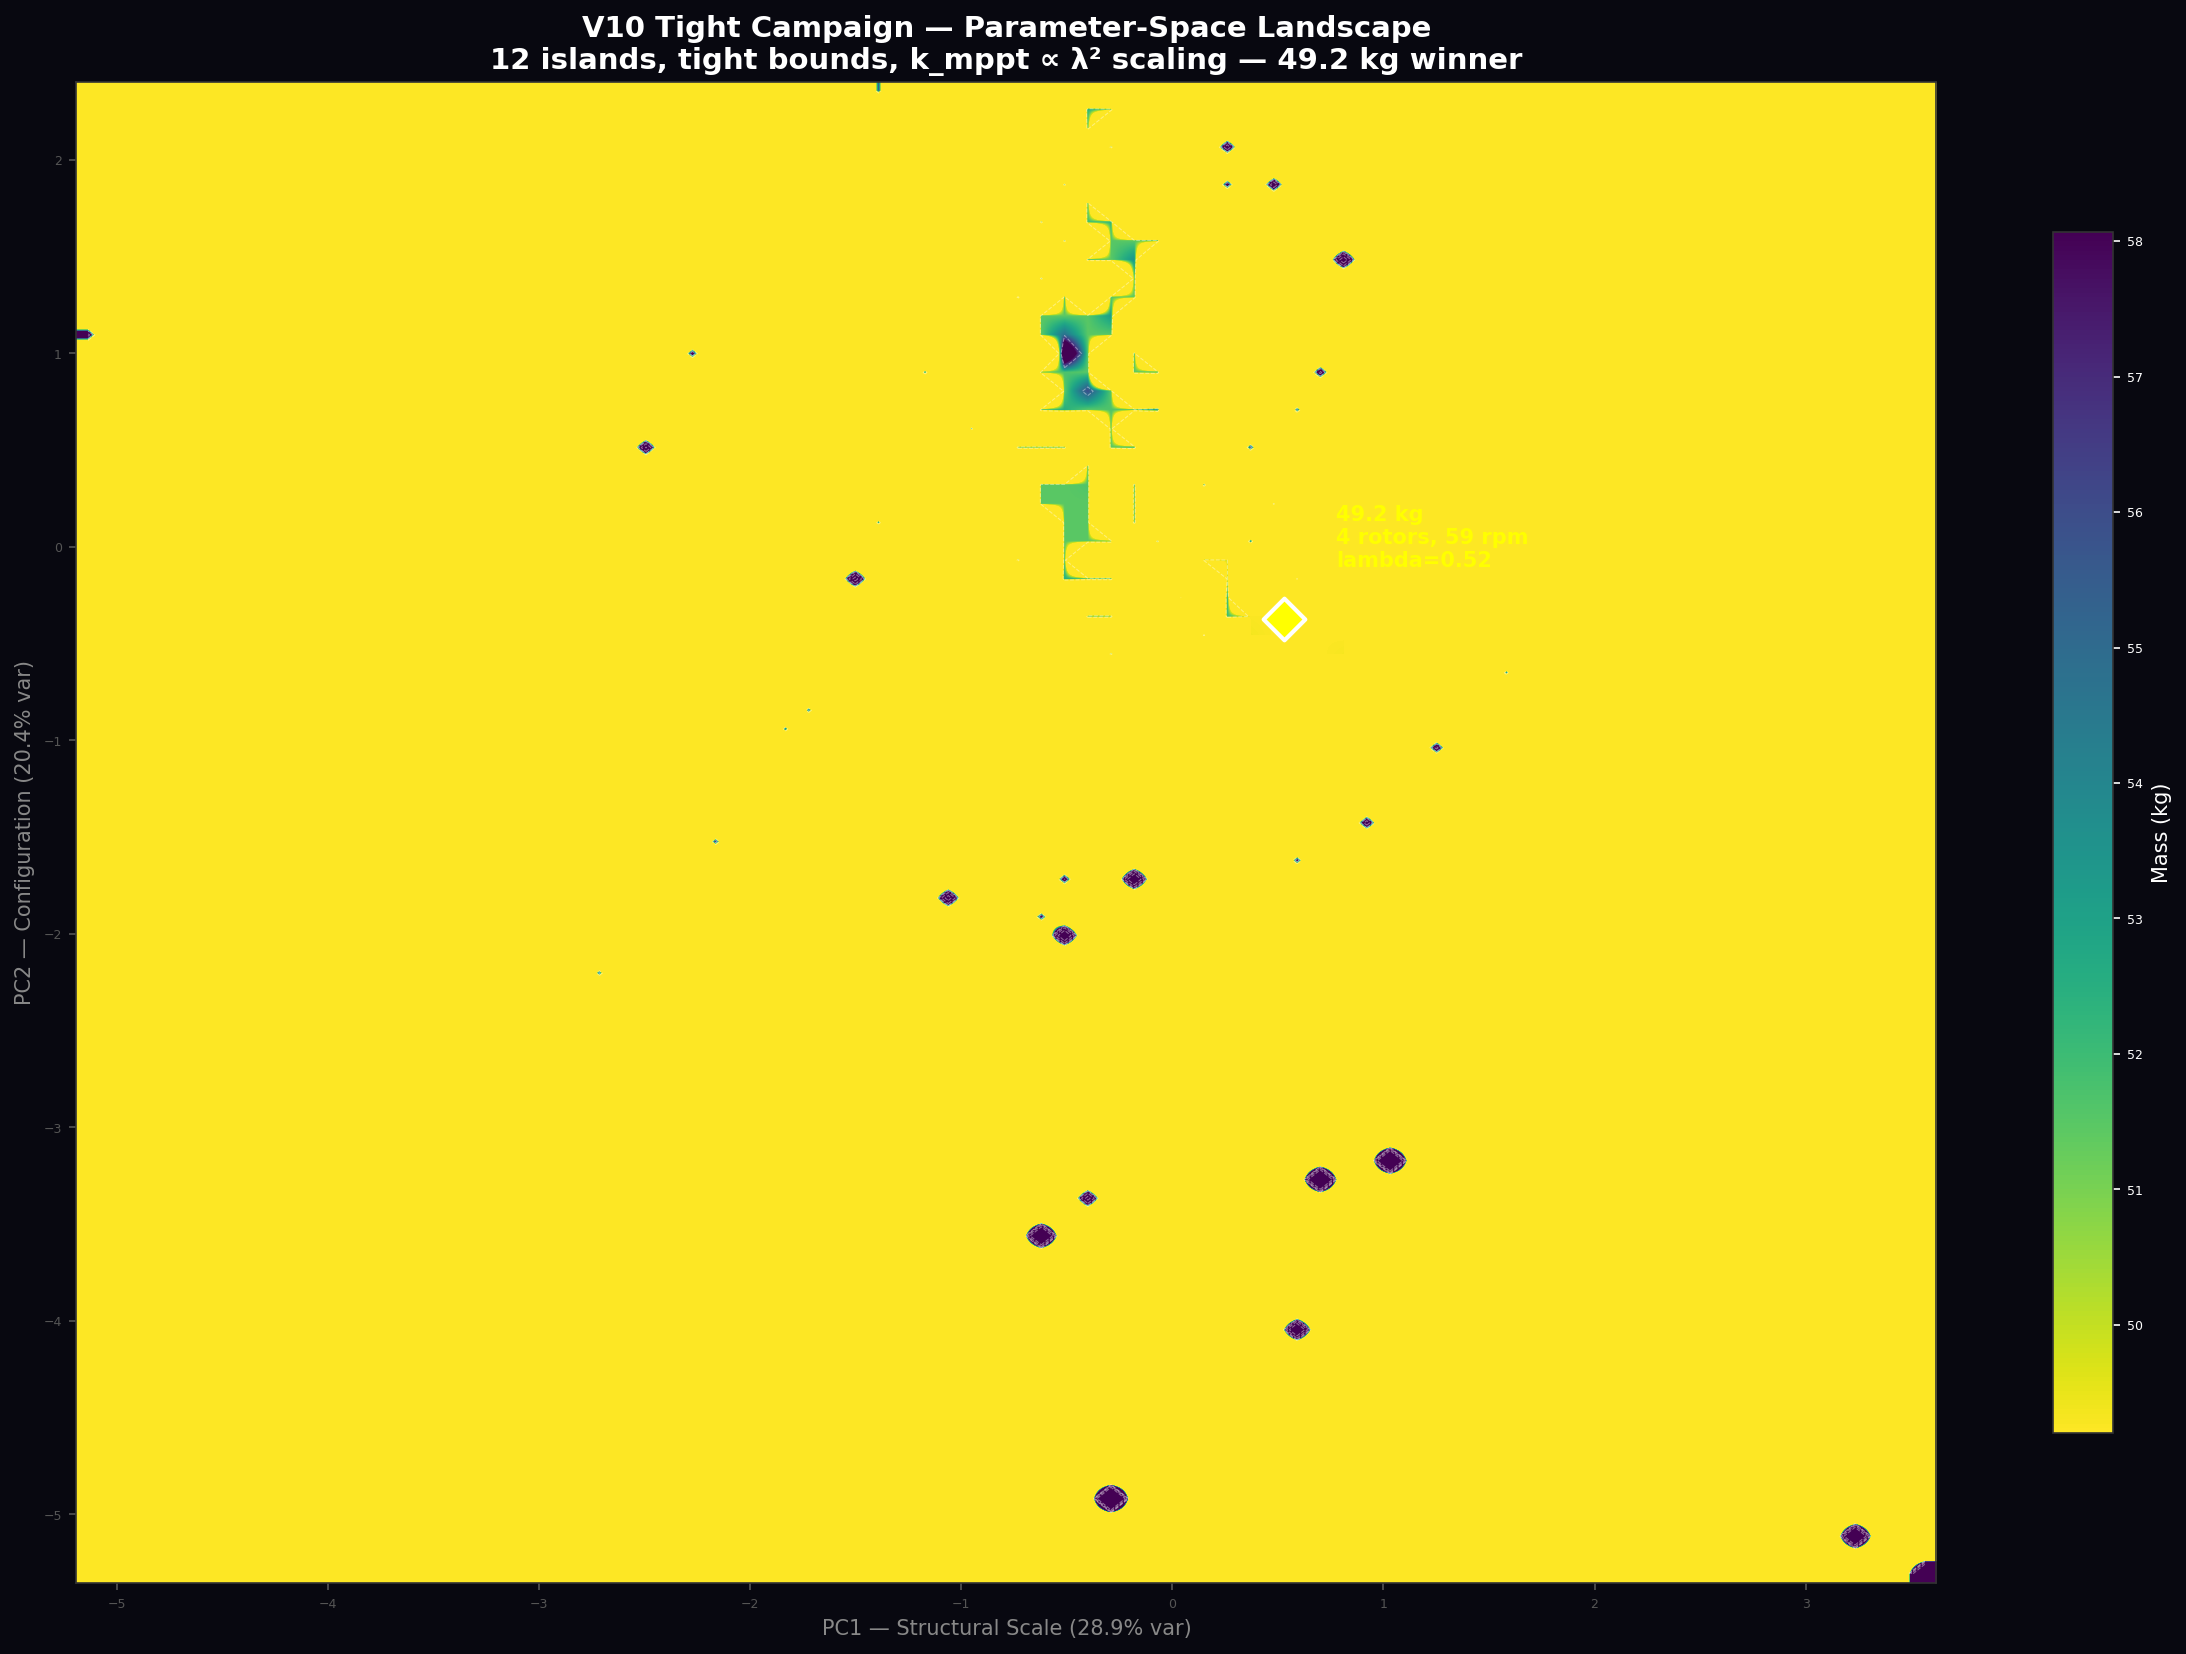
\includegraphics[width=0.85\textwidth]{v10-tight-landscape.png}
\caption{V10 Tight campaign: PCA projection of the 14-dimensional design space. Each point is a design evaluation, coloured by total airborne mass (dark purple = lightest). White dashed contours at 50 and 65\,kg. Yellow diamond = campaign winner at 49.2\,kg. PC1 (28.9\% variance) captures structural scale; PC2 (20.4\%) captures configuration choice.}
\label{fig:pca}
\end{figure}

\begin{figure}[htbp]
\centering
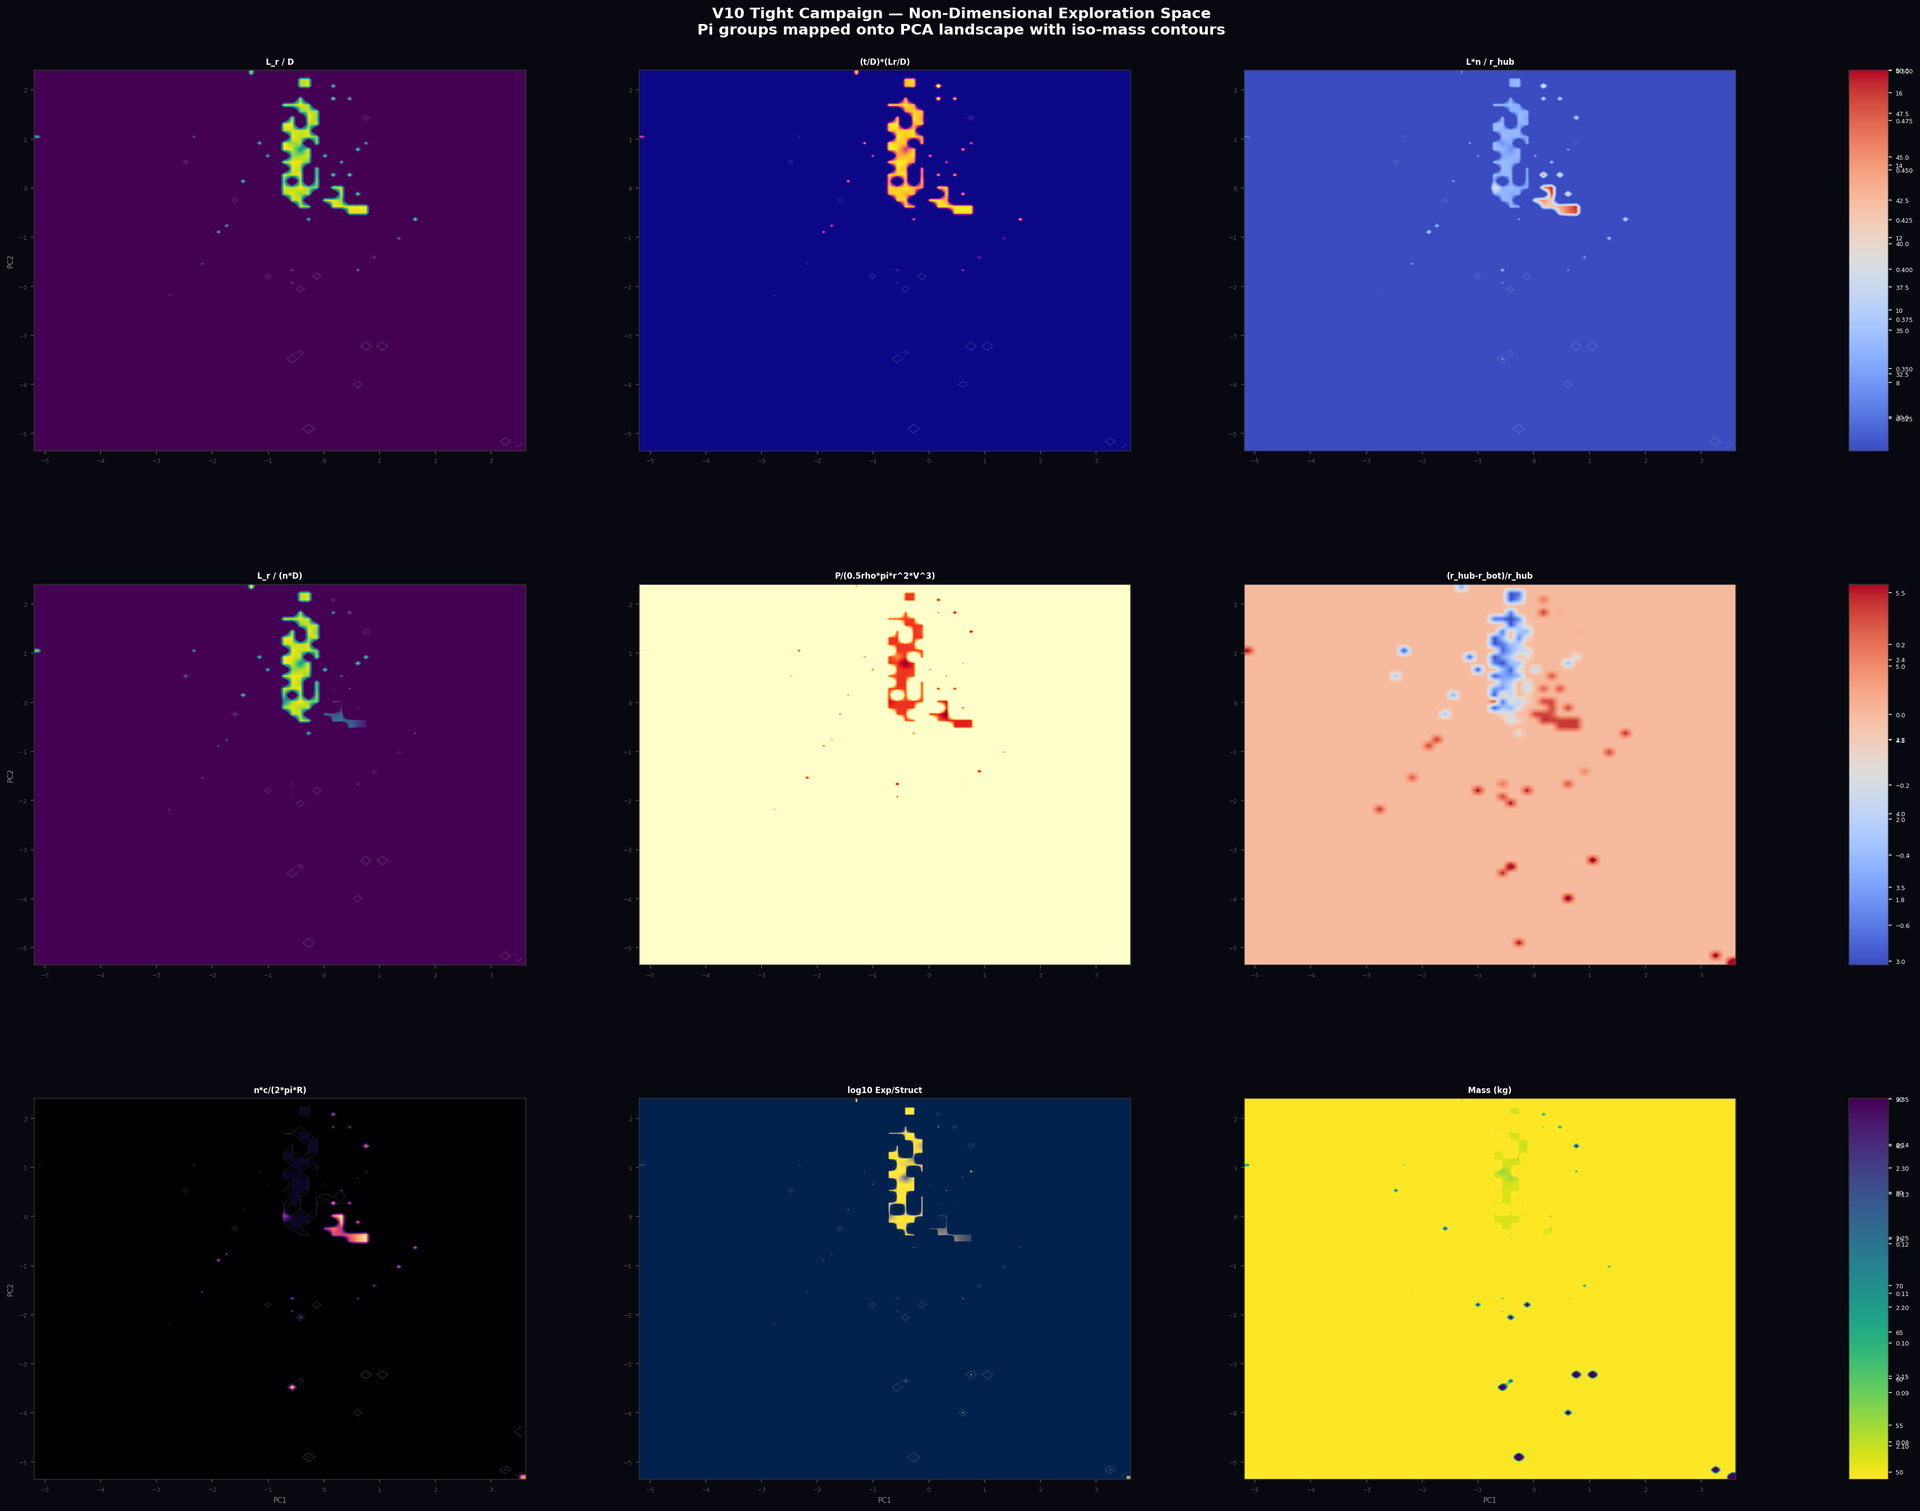
\includegraphics[width=0.85\textwidth]{v10-tight-nondim.png}
\caption{Non-dimensional physics atlas: nine Pi groups colouring the PCA design space, revealing the physical mechanisms behind the 49.2\,kg optimum. Panels: beam slenderness, beam efficiency, TRPT aspect ratio, ring packing, power loading, ring taper, rotor solidity, expansion/structural ratio, mass.}
\label{fig:nondim}
\end{figure}

% ══════════════════════════════════════════════════════════════════════════════
\section{Conclusion}
% ══════════════════════════════════════════════════════════════════════════════

TRPT kite turbines with multi-rotor expansion represent a material-efficient path to utility-relevant airborne wind energy.
The KTD.jl framework has quantified the achievable mass range (49--61\,kg at 50\,kW), identified the 4.2$\times$ static--dynamic gap as the critical modelling challenge, and established left-flank overspeed as the viable operating architecture.

The gaps that remain---mid-fidelity aerodynamics, wake interaction modelling, hardware validation, and dynamic-aware optimisation---are precisely the areas where the groups addressed in this report have world-leading expertise.
We invite collaboration on any of the proposals outlined above, and we are prepared to lead or join consortium grant applications to fund dedicated research time.

The simulator is open-source, the test suite is green, and the decisions are documented.
The next step is a conversation.

\vspace{18pt}
\begin{center}
\textit{Rod Read}\\
Windswept \& Interesting Ltd, Stornoway, Scotland\\
\texttt{rod@windswept.energy}
\end{center}

% ══════════════════════════════════════════════════════════════════════════════
% REFERENCES
% ══════════════════════════════════════════════════════════════════════════════

\begin{thebibliography}{99}

\bibitem{tulloch2023}
Tulloch, O., Yue, H., Kazemi Amiri, A.M.\ and Read, R. (2023).
A tensile rotary airborne wind energy system---modelling, analysis and improved design.
\emph{Energies}, 16(6), 2610.

\bibitem{tulloch2021}
Tulloch, O. (2021).
\emph{Tensile Rotary Power Transmission Design}.
PhD Thesis, University of Strathclyde.

\bibitem{jamieson2020}
Jamieson, P. (2020).
Top-level rotor optimisations using actuator disk theory.
\emph{Wind Energy Science}, 5, 807--818.

\bibitem{vanleersum2023}
van Leersum, D. (2023).
TRPT scaling analysis---internal report for Windswept \& Interesting Ltd.
Unpublished.

\bibitem{chen2026}
Chen, Z., Yue, H., Kazemi, A.\ and Read, R. (2026).
Power efficiency analysis of a rotary kite airborne wind energy system.
\emph{Proceedings of the 11th International Airborne Wind Energy Conference (AWEC 2026)}, Porto, Portugal.

\bibitem{amjad2026}
Amjad Zulfazli, M.M., Yue, H., Carroll, J.\ and Chen, Z. (2026).
Scalability analysis of a rotary kite airborne wind energy system with tensile rotary power transmission.
\emph{Proceedings of the 11th International Airborne Wind Energy Conference (AWEC 2026)}, Porto, Portugal.

\bibitem{leuthold2019}
Leuthold, R., Crawford, C., Gros, S.\ and Diehl, M. (2019).
Engineering wake induction model for axisymmetric multi-kite airborne wind energy systems.
\emph{Wake Conference 2019}.

\bibitem{leuthold2017}
Leuthold, R., Gros, S.\ and Diehl, M. (2017).
Induction in optimal control of multiple-kite airborne wind energy systems.
\emph{IFAC-PapersOnLine}, 50(1), 153--158.

\bibitem{leuthold2026}
Leuthold, R., Crawford, C., Gros, S.\ and Diehl, M. (2026).
Trajectory tracking in AWE optimal control with a rigidly-convected, lifting-line vortex model.
\emph{Proceedings of the 11th International Airborne Wind Energy Conference (AWEC 2026)}, Porto, Portugal.

\bibitem{diehl2026}
Diehl, M., Harzer, J.\ and De Schutter, J. (2026).
Vertical airborne wind energy farms based on dual-wing systems.
\emph{Proceedings of the 11th International Airborne Wind Energy Conference (AWEC 2026)}, Porto, Portugal.

\bibitem{beaupoil2026}
Beaupoil, C.\ and Weyel, F. (2026).
Autogyro pumping mode rotary AWE system---design and control of a servo flap cyclic pitch actuated rotor.
\emph{Proceedings of the 11th International Airborne Wind Energy Conference (AWEC 2026)}, Porto, Portugal.

\bibitem{kheiri2018}
Kheiri, M., Bourgault, F.\ and Iosilevskii, G. (2018).
Power limit and its governing factors for crosswind kite systems.
\emph{Journal of Aircraft}, 55(4), 1534--1548.

\bibitem{carceller2022}
Carceller Candau, J. (2022).
Dynamic analysis of a rotary airborne wind energy system.
MSc Thesis, Universitat Polit\`ecnica de Catalunya.

\bibitem{ktd_decisions2026}
Read, R. (2026).
\texttt{KiteTurbineDynamics.jl}---\texttt{DECISIONS.md} (architectural decision log).
\url{https://github.com/rodread/KiteTurbineDynamics.jl}

\bibitem{harzer2026}
Harzer, J., Polkl\"aser, K.S., Diehl, M.\ and Moormann, D. (2026).
Multi-wing AWE research project: goals and progress.
\emph{Proceedings of the 11th International Airborne Wind Energy Conference (AWEC 2026)}, Porto, Portugal.

\end{thebibliography}

\end{document}
